%% ****** Start of file auguide.tex ****** %
%%
%%   This file is part of the AIP distribution of substyles for REVTeX 4.1
%%   For version 4.1r of REVTeX, August 2010
%%
%%   Copyright (c) 2009,2010 American Institute of Physics
%%
\listfiles
\documentclass{article}
% \documentclass[%
%  reprint,%
% %secnumarabic,%
%  amssymb, amsmath,%
%  aip,jap,%
% %groupedaddress,%
% %frontmatterverbose,
% ]{revtex4-1}

% \usepackage{docs}%
\usepackage{graphicx}%
\usepackage{epstopdf}
\usepackage{color}
\usepackage{algorithm}
\usepackage[noend]{algpseudocode}
\usepackage{minted}

\makeatletter
\def\BState{\State\hskip-\ALG@thistlm}
\makeatother

\usepackage{amsmath}


\usepackage{bm}%
\usepackage[colorlinks=true,linkcolor=blue]{hyperref}%
%\nofiles
\expandafter\ifx\csname package@font\endcsname\relax\else
 \expandafter\expandafter
 \expandafter\usepackage
 \expandafter\expandafter
 \expandafter{\csname package@font\endcsname}%
\fi
\hyphenation{title}

\begin{document}

\title{Asynchronous Stochastic Gradient Descent}%
\author{Vivek Subramaniam, Ashish Sharma, Dylan Pederson}
%\email{vivek91@utexas.edu}
%\email{dpederson@utexas.edu}


\maketitle

 


\section{Introduction}\label{sec:intro}
Asynchronous parallel stochastic optimization algorithms are an attractive option for approximately solving optimization problems on large data sets. If the cost function can be cast as

\begin{equation}\label{eqn:erm}
	f(x) = \frac{1}{n}\sum_{i=1}^n f_i(x)
\end{equation}

then an approximate gradient $g_x$ can be calculated in a shorter amount of time than the full gradient. Furthermore, if the functions $f_i(x)$ depend only on a subset of the coordinates $x_j$ (i.e. the gradient of $f_i$ is sparse), then applying the approximate gradients can be done quickly. As long as the approximate gradient has the property that $\mathbf{E}[g_x] = \nabla f(x)$, this scheme can be shown to converge on average to the true optimum. The algorithm called HOGWILD! implements asynchronous SGD \cite{niu2011}. 

\begin{algorithm}
	\caption{HOGWILD!}\label{hogwild!}
	\begin{algorithmic}[1]
	\While {number of sampled hyperedges $\le$ T} in parallel
	\State sample a random hyperedge s
	\State $[\hat{x}]_s$ = an inconsistent read of the shared variable $[x]_s$
	\State $[u]_s = -\gamma g([\hat{x}]_s, s)$
	\For {$v \in s$}
		\State $[x]_v = [x]_v + [u]_v$
	\EndFor
	\EndWhile
	\end{algorithmic}
\end{algorithm}
 
According to \cite{horia2016}, HOGWILD! with a step size $\gamma = \frac{\epsilon m}{2 M^2}$ will reach error $\epsilon$ in 

\begin{equation}
	T \ge O(1)\frac{M^2 log(\frac{a_0}{\epsilon})}{\epsilon m^2}
\end{equation}

with a function that is $m$-strongly convex with initial guess distance $M^2$. This error bound shows that HOGWILD! achieves linear speedup, and can be further improved if the step size is diminished each time step. 

In this work we will utilize the HOGWILD! algorithm to solve a sparse logistic regression problem

\begin{equation}\label{eqn:logreg}
	\min_{\beta} \frac{1}{n} \sum_{i=1}^n(\beta_{y_i}^{T}x_i + log \sum_{j=1}^C e^{-\beta_j^T x_i}) + \mu ||\beta||^2
\end{equation}

where 

\begin{equation}\label{eqn:y_i}
	y_i \in \{1,2,...,C\}
\end{equation}

is the classification label of the data point $i$, and 

\begin{equation}\label{eqn:y_i}
	\beta = [\beta_1, \beta_2, ..., \beta_C]^T
\end{equation}

is the vector of concatenated solutions for each classification. To compute the stochastic gradient, we reformulate the problem as follows

\begin{equation}\label{eqn:logreg1}
	\min_{\beta} \frac{1}{n} \sum_{i=1}^n(\beta_{y_i}^{T}x_i + log \sum_{j=1}^C e^{-\beta_j^T x_i}) + \mu ||\beta||^2
\end{equation}
\begin{equation}\label{eqn:logreg2}
	= \min_{\beta} \frac{1}{n} \sum_{i=1}^n(\beta_{y_i}^{T}x_i + log \sum_{j=1}^C e^{-\beta_j^T x_i}) + \frac{1}{n}\sum_{i=1}^n \mu ||\beta||^2
\end{equation}
\begin{equation}\label{eqn:logreg3}
	= \min_{\beta} \frac{1}{n} \sum_{i=1}^n(\beta_{y_i}^{T}x_i + log \sum_{j=1}^C e^{-\beta_j^T x_i} + \mu ||\beta||^2)
\end{equation}
\begin{equation}\label{eqn:logreg4}
	= \min_{\beta} \frac{1}{n} \sum_{i=1}^n(\beta_{y_i}^{T}x_i + log \sum_{j=1}^C e^{-\beta_j^T x_i} + \mu \sum_{j=1}^C \beta_j^T\beta_j)
\end{equation}

which allows us to then identify $f_i(\beta)$ as in \ref{eqn:erm}. 

\begin{equation}\label{eqn:f_i}
	f_i(\beta) = \beta_{y_i}^{T}x_i + log \sum_{j=1}^C e^{-\beta_j^T x_i} + \mu \sum_{j=1}^C \beta_j^T\beta_j
\end{equation}

We can then take the partial gradients

\begin{equation}\label{eqn:gradient}
	\nabla_{\beta_j} f_i(\beta) = \begin{cases}
								  x_i + 2\mu\beta_j - x_i\frac{e^{-\beta_j^T x_i}}{\sum_{j=1}^C e^{-\beta_j^T x_i}} & (j = y_i) \\
								  2\mu\beta_j - x_i\frac{e^{-\beta_j^T x_i}}{\sum_{j=1}^C e^{-\beta_j^T x_i}} & (j \neq y_i)
								  \end{cases}
\end{equation}

Note here that if $x_i$ is sparse, and $\beta_j$ starts off sparse, then the iterates of $\beta$ are sparse. We can see this by inserting the gradient update into the update equation.


\begin{equation}\label{eqn:update}
	\beta_j^+ = \begin{cases}
								  \beta_j(1-2\gamma\mu) - \gamma x_i(1-\frac{e^{-\beta_j^T x_i}}{\sum_{j=1}^C e^{-\beta_j^T x_i}}) & (j = y_i) \\
								  \beta_j(1-2\gamma\mu) - \gamma x_i(-\frac{e^{-\beta_j^T x_i}}{\sum_{j=1}^C e^{-\beta_j^T x_i}}) & (j \neq y_i)
								  \end{cases}
\end{equation}

From \ref{eqn:update} it becomes obvious that the support of $\beta_j^+$ is a union of the support of $\beta_j$ and $x_i$. Asynchronous SGD proceeds with each process choosing a random index (hyperedge) $[i]$ from a uniform distribution to calculate an approximate gradient $g_x = \nabla f_{[i]}$. For our purposes, we assume 2 classes ($C=2$) and $n$ data points. The dataset in this report comes from the libSVM  \textbf{rcv1} data, which contains $20,242$ data points with a sparse subset of $47,236$ features \cite{libSVM}, in which the dataset is large with sparse sets of features for each data point. 

An improvement upon SGD, called Variance Reduced SGD (SVRG), can be used to get faster convergence, while still reducing the computational cost of each iteration. In SVRG, the approximate gradient is changed to be 

\begin{equation}\label{eqn:svrg_grad}
	g_x = \nabla f_{[i]}(\beta) - \nabla f_{[i]}(\alpha) + \nabla f(\alpha)
\end{equation}

where $\alpha$ is a solution vector at a previous time step. It can be shown that $\mathbf{E}[g_x] = \nabla f(\beta)$ and that the variance of this gradient is smaller than that of the SGD gradient. In SVRG, the full gradient $\nabla f(\alpha)$ is calculated every $m$ time step. Thus it achieves a sort of balance between GD and SGD in terms of convergence and computational cost. We will explore parallelizing both SGD and SVRG.

\section{Implementation}
We implement our code in C++, using the OpenMP framework for shared memory parallelization. OpenMP works to our advantage with its support for atomic writes and locks, so that we may explore the effect of synchronization on the SGD problem. Coding elements of the project include a file parser to access data points in the dataset, a sparse matrix representation (compressed row format), and a sparse vector object to take advantage of the sparse iterates produced by the algorithm (and the sparsity of the data features). Analysis elements of the project include analyzing parallel algorithm speedup and cost function value (convergence) for each iteration.

\section{Results}

\subsection{SGD}
In this test, we use a total of $10,000$ iterations with a constant step size $\gamma$ starting at $5$ and decreasing stepwise at $500$ and $5000$ iterations (see Code section for detail).

\begin{figure}[!htbp]
	\centering
	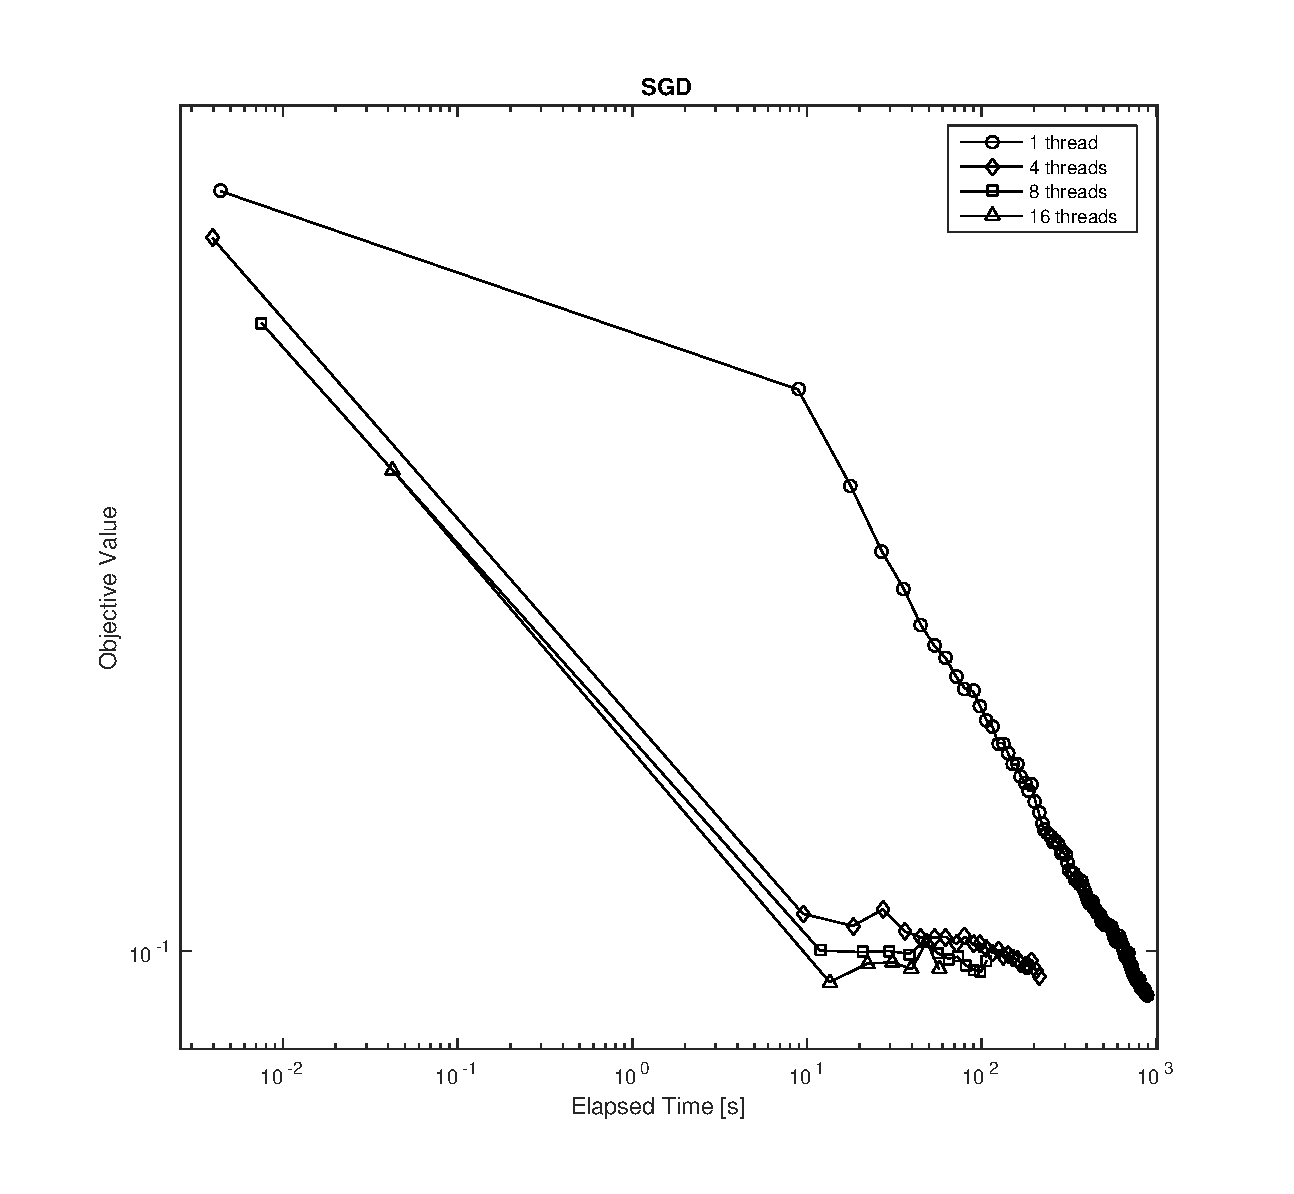
\includegraphics[scale=0.5]{figs/sgd_objective.eps}
	\caption{Evolution of the objective function value over time}
	\label{fig:sgd_objective}
\end{figure}

\begin{figure}[!htbp]
	\centering
	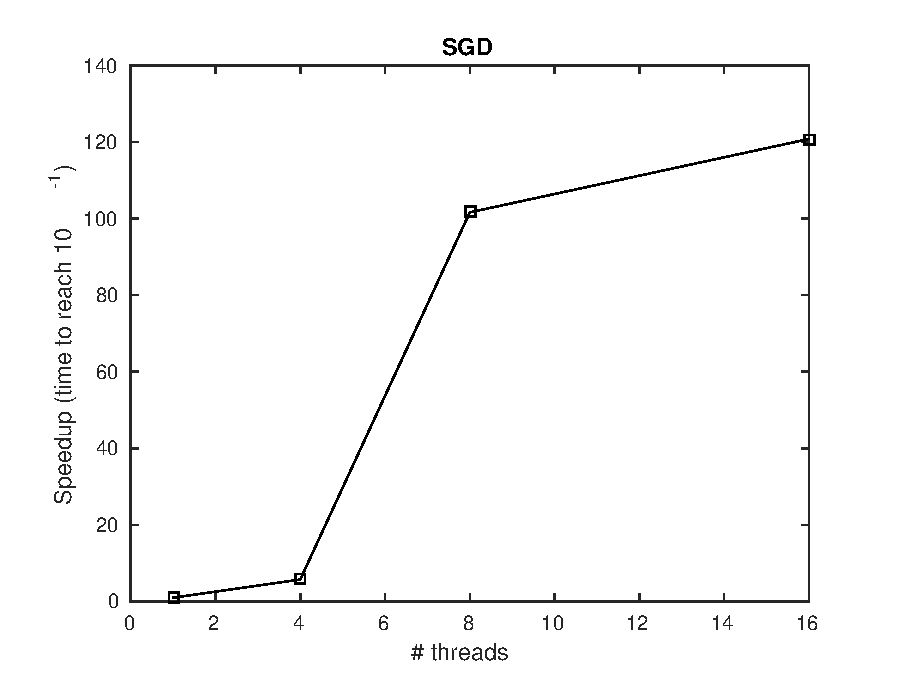
\includegraphics[scale=0.5]{figs/sgd_speedup.eps}
	\caption{Parallel speedup for the Stochastic Gradient Descent method}
	\label{fig:sgd_speedup}
\end{figure}

The values in Figure \ref{fig:sgd_speedup} are quite large and probably inaccurate because of the selected objective function value of $10^{-1}$. A smaller objective function value would require exponentially more iterations, but would probably be more accurate. But still, this shows that parallelizing SGD gives a good (approximately linear) speedup.

\subsection{SVRG}
In this test, we use an iterval $m=400$ iterations, and again a total of $10,000$ iterations with the same step size schedule as SGD above.

\begin{figure}[!htbp]
	\centering
	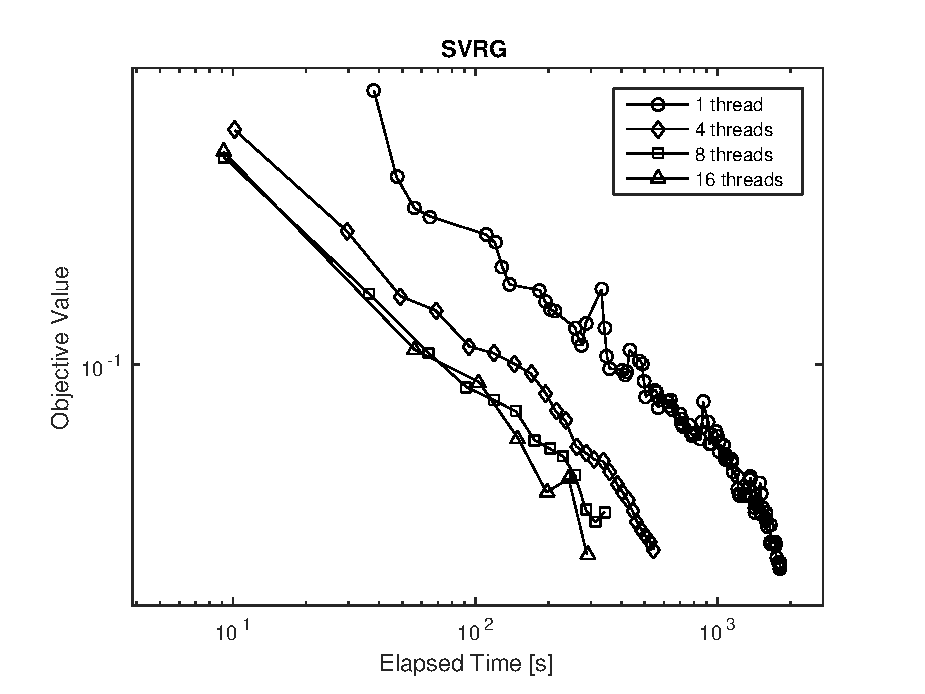
\includegraphics[scale=0.5]{figs/svrg_objective.eps}
	\caption{Evolution of the objective function value over time}
	\label{fig:svrg_objective}
\end{figure}

\begin{figure}[!htbp]
	\centering
	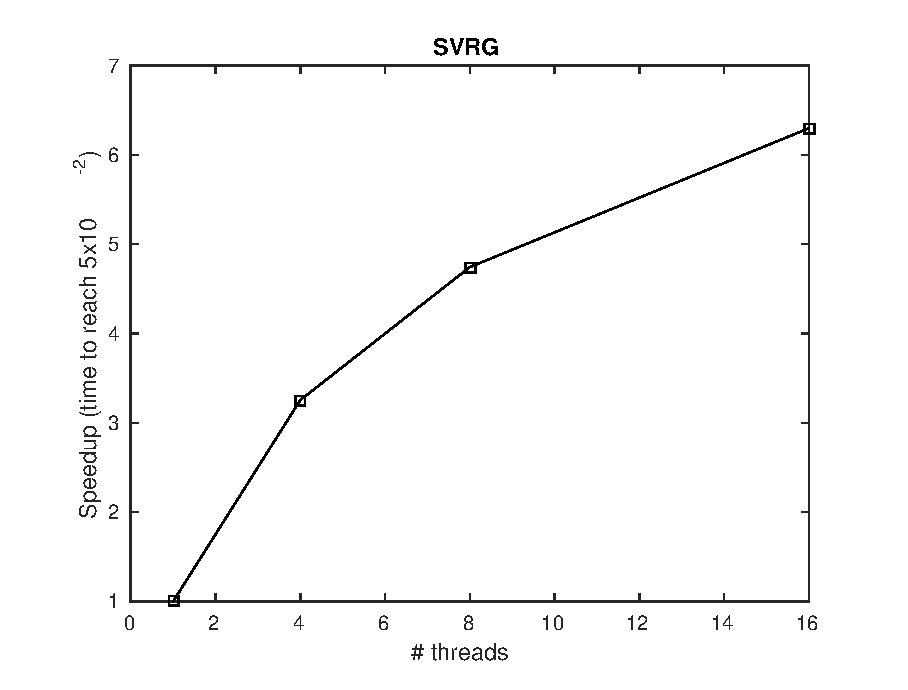
\includegraphics[scale=0.5]{figs/svrg_speedup.eps}
	\caption{Parallel speedup for the Stochastic Gradient Descent method}
	\label{fig:svrg_speedup}
\end{figure}

Figure \ref{fig:svrg_speedup} shows that parallel SVRG achieves approximately linear speedup up to 16 threads. This is encouraging for larger scale problems that can benefit from more threads. 


\begin{figure}[!htbp]
	\centering
	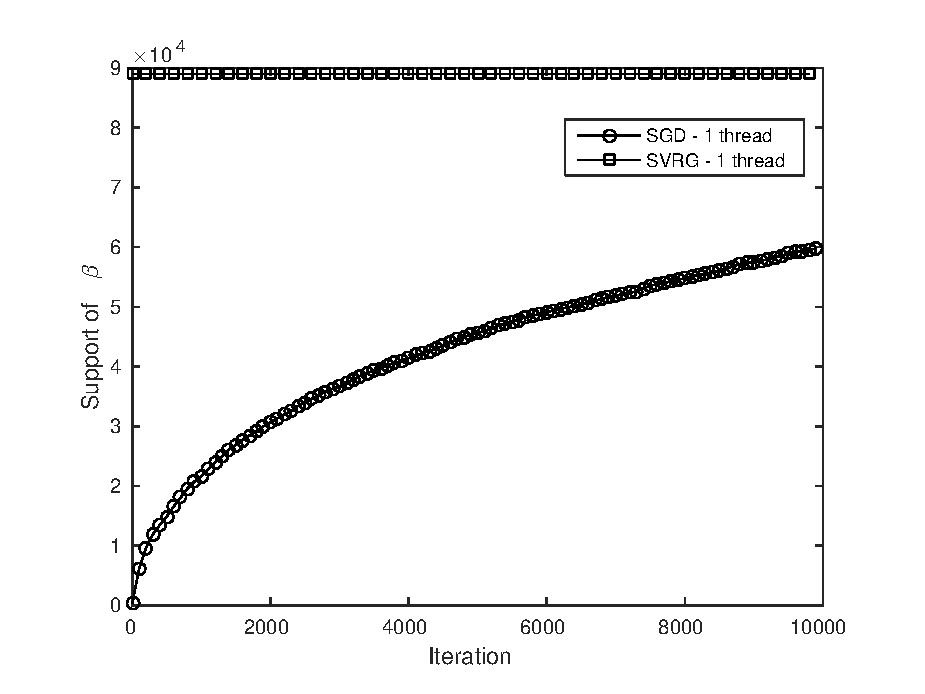
\includegraphics[scale=0.5]{figs/sup_beta.eps}
	\caption{Support of $\beta$ during the descent. As expected, SGD has a gradually increasing support, while SVRG has a fairly large and constant support from the beginning}
	\label{fig:support_beta}
\end{figure}

\section{Conclusions}
Parallelizing SGD and SVRG is an easy and efficient way to speed up computation time of learning algorithms. SGD produces sparse iterates that can be taken advantage of, while SVRG does not produce sparse iterates (\cite{horia2016} introduces a \textit{sparse} version of SVRG, dubbed KroMagnon). Parallel speedup is shown to be fairly linear up to 8 threads on the \textbf{rcv1} logistic regression data set. Future improvements might be to implement a sparse SVRG similar to KroMagnon, and to enable reading of larger datasets that don't fit into shared memory on one node.

\bibliography{asynchsgd}%{}
\bibliographystyle{plain}


\section{Code}

\inputminted{c++}{../grad_class.h}


\end{document}

